\subsection{M.PC.5 - EAC (Estimated at Completion)}
\begin{figure}[H]
    \centering
    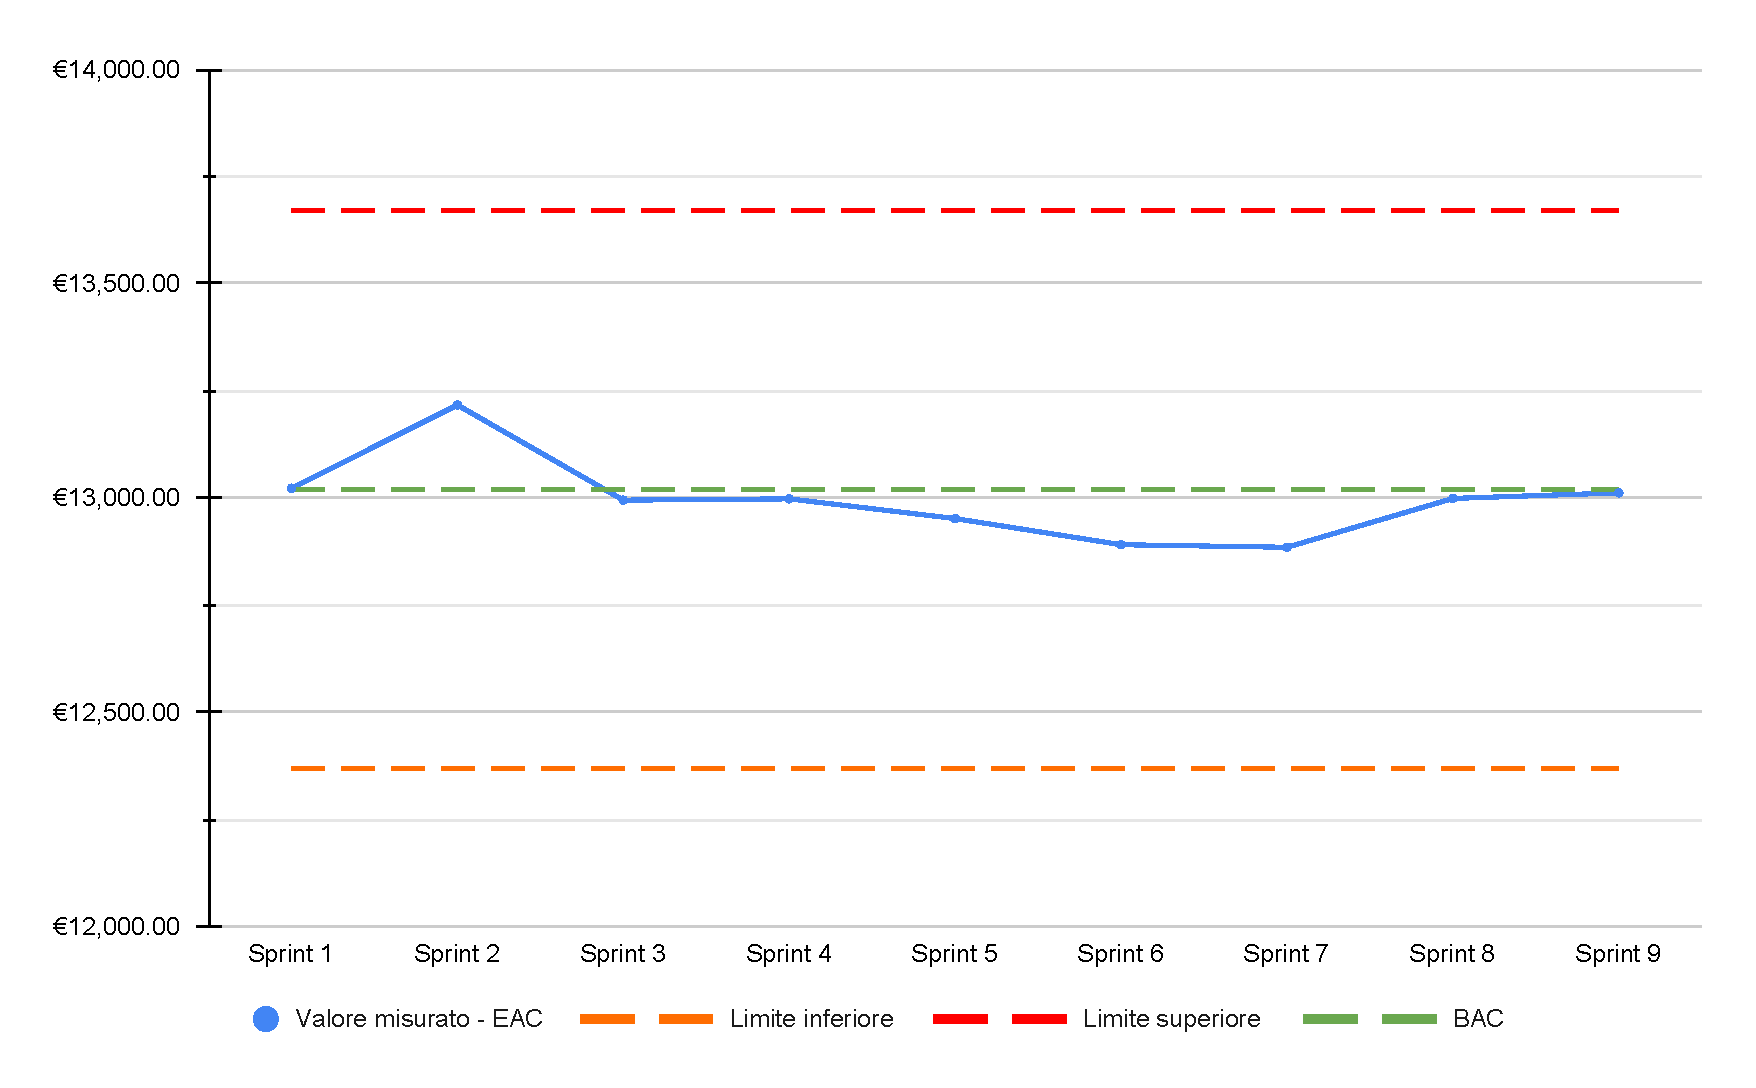
\includegraphics[width=\textwidth]{assets/stima_a_finire.pdf}
    \caption{M.PC.5 - EAC (Estimated at Completion)}
\end{figure}

\par Nella fase iniziale del progetto, l'EAC (costo sostenuto + stima costo ancora da sostenere) è rimasto in linea con il BAC (valore iniziale previsto), con l’unica eccezione rappresentata dal secondo \glossario{sprint}. Durante la pianificazione del secondo sprint, infatti, il gruppo ha riscontrato delle carenze strutturali nella documentazione. Pertanto, gli sforzi del team si sono concentrati sulla rettifica dei documenti prodotti fino a quel momento. In particolare, la riorganizzazione dell'\AdR, del \PdP\ (con l'aggiunta della gestione dei rischi e del preventivo “a finire”) e dei verbali (con l’aggiunta della tabella “Todo”), hanno richiesto un impegno maggiore del previsto. Inoltre, lo studio dei nuovi strumenti e tecnologie (tra cui \glossario{Jira}, \glossario{YAML} e \glossario{txtai}) ha rallentato l’avanzamento dei lavori, mantenendo però i costi elevati. Nonostante il budget stimato per la realizzazione del progetto abbia superato il BAC, il team ha comunque rispettato il range di tollerabilità stabilito. A partire dal terzo sprint, invece, la stima del budget è risultata inferiore rispetto al BAC, avvicinandosi a quest’ultimo nell’ottavo sprint (coincidente con la sessione di esami). L’andamento del grafico denota come le azioni preventive e correttive impiegate dal team abbiano avuto esito positivo, garantendo il rispetto del budget nonostante il cambio tecnologico avvenuto nel quinto sprint.